\chapter{Models for Adaptive Testing}


We remind, as was mentioned in the section~\ref{sec:CATprocess}, the process of an adaptive test.
\begin{enumerate}
	\item The next question to be asked is selected.
	\item The question is asked and a result is obtained.
	\item The result is inserted into the model.
	\item The model (i.e. our estimation about the student) is updated with the result.
	\item (optional) Subsequent answers are estimated / the skill of the student is estimated
\end{enumerate}
In this section we will take a closer look on the model structure for different approaches. Also we will discuss the question selection from step 1 of the list above. Insertion to the model (step 3) and consequent update (steps 4 and 5) of the model is always done with respective standard tools for particular model and will not be extensively discussed here.

\section{Building Models with the Help of IRT}
\label{sec_IRT}
The beginning of Item Response Theory (IRT) appears about 5 decades ago (1968 - Statistical Theories of Mental Test Scores / Lord, Novick -- 1960 - Probabilistic Models for Some Intelligence and..., Rash). This approach is different form the Classical Test Theory (CTT) and it has getting scientific attention ever since [CITACE - str 152].  IRT allows more specific measurement of certain abilities of an examinee. Internationally, there is a large amount of tests adapting this concept. It has stronger assumptions but it also provide stronger results. Nevertheless its spread is not as high as could have been expected. This smaller impact might be caused by the fact that there is a requirement for a stronger statistical and theoretical preparation of a test creator than in the CTT. \textbf{In the Czech Republic there is just a few tests which use this concept. []} 

IRT expects student to have an ability (skill) which directly influences his/her chance of answering a question correctly\footnote{There are variants of multidimensional IRT model where it is possible to have more then one latent variable but in this section we are going to discuss only models with one latent variable.}. This ability is called latent ability or latent trait $\theta$. Every question of the IRT model has associated item response function (IRF) which is a probability of a successful answer given $\theta$. There are more variants to the shape of this IRF but most commonly a 3 parametric model is used (often called 3PL). These parameters reshape a standard logistic function. The resulting IRF, as the probability of a correct answer to \textit{i-th} with the ability of $\theta$, is given by a formula
\begin{equation}
p_i(\theta) = c_i + \frac{1-c_i}{1+e^{-a_i(\theta-b_i)}}
\label{eq:IRF}
\end{equation}
where $c_i$ is a parameter for guessing, $a_i$ sets the scale of the question (this sets its discrimination ability - more steep curve better differentiate between students), $b_i$ is the difficulty of the question (horizontal position of the curve in the space). An example of typical IRFs is shown in the Figure~\ref{pic:IRFs} and the Table~\ref{tab:IRFs} shows their parameters.\\
IRFs are created during the learning procedure of the model from collected data as most likelihood estimates of their parameters.

\begin{figure}
  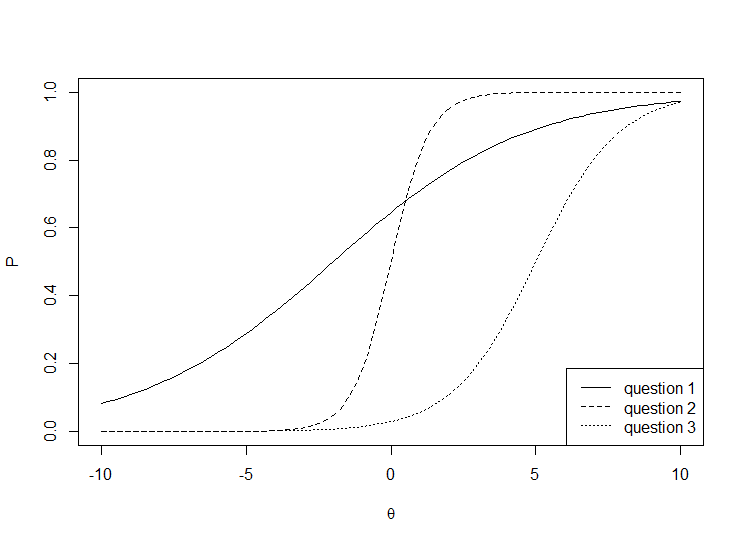
\includegraphics[width=0.8\columnwidth]{obr/irfs.png}%
  \caption{Item Response Functions}%
	\label{pic:IRFs}%
\end{figure}
\begin{table}%
	\begin{tabular}{lccc} \hline
		Question & a & b & c \\ \hline
		1 & -2 & 0.3 & 0\\
		2 & 0 & 1.5 & 0\\
		3 & 5 & 0.7 & 0\\
	\hline
  \end{tabular}
  \caption{IRFs' parameters}%
	\label{tab:IRFs}%
\end{table}
  


\subsection{Adaptive Test Procedure}
Building CAT model with IRT is very straightforward. IRT itself, as was described above, is in the form prepared to be used for CAT. With the model fitted from sample data we have IRFs for every question. In every phase of the test we can compute an estimate of the latent skill $\theta$ based on answers $x$: $p(\theta|x)$. For this estimations Empirical Bayes or Multiple Imputation methods of IRT are used. Knowing the value of the latent skill we know probabilities of correct answers to every question $p_i(\theta)$ and incorrect answers $q_i(\theta)$\footnote{With 3 parametric model these two numbers do not necessarily sum to 1}. More importantly, we are able to calculate the information provided by asking the question. This is called item information and it is given by the formula
$$I_i(\theta)=\frac{(p_i'(\theta))^2}{p_i(\theta)q_i(\theta)}$$
where $p_i'$ is the derivation of the item response function $p_i$. There is an example of typical item information functions (with the same parameters of items as in the Table~\ref{tab:IRFs}) in the Figure~\ref{pic:IG}. This item information provide one, and most straightforward, way of the next question selection. In every step the question $X^*$ which is selected is one with the highest item information. 
$$X^*(\theta) = \arg\max_i I_i(\theta)$$
\textbf{This approach minimizes the standard error of the test procedure.}

\begin{figure}%
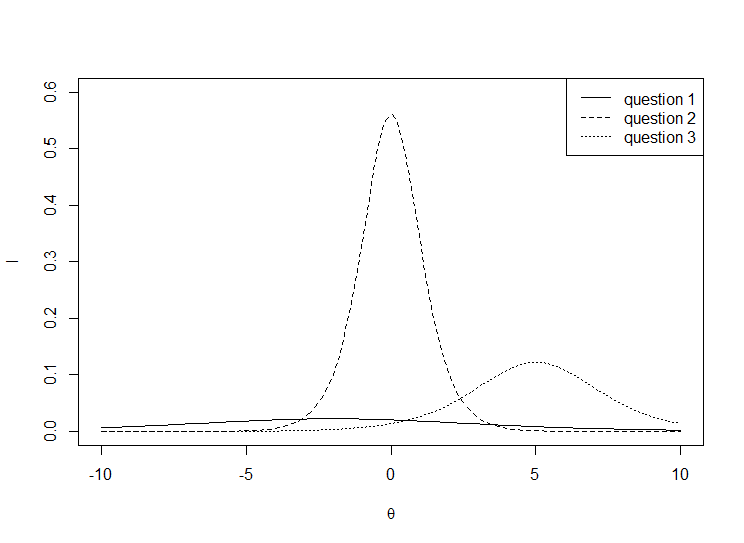
\includegraphics[width=0.8\columnwidth]{obr/IIs.png}%
\caption{Item Information Functions}%
\label{pic:IG}%
\end{figure}

\section{Building Models with the Help of BN}

In this section we go over the basic definitions of Bayesian networks. More theory can be found in []. This section is focused on creation Bayesian networks models for CAT.

Bayesian network is a probabilistic graphical model, a conditional independence structure. It consists of the following: 
\begin{itemize}
	\item a set of variables (nodes),
	\item a set of edges,
	\item a set of conditional probabilities.
\end{itemize}
Edges between variables have to form a directed acyclic graph (DAG). Each variable has a list of mutually exclusive possible states. The conditional probability distribution is defined for each variable conditioned by its parents (variable $A$ with parents $B_1$,$B_2$,...,$B_n$ has the conditional probability table ${P(A|B_1,B_2,...,B_n)}$)\footnote{Note that the variables with no parents have the table in the form $P(A)$}. 

To build a model for adaptive testing as a BN we need to perform 3 steps.
\begin{enumerate}
	\item Describe nodes of the BN
	\item Describe connections between nodes
	\item Initialize conditional probability tables
\end{enumerate}
 
\subsubsection{TYPES OF NODES}
We will divide nodes of a BN into more specific sets. 
\begin{itemize} 
\item A set of $n$ variables we want to estimate $\{S_1,\ldots,S_n\}$. 
We will call them skills or skill variables. We will use symbol $S$ to denote the multivariable $(S_1,\ldots,S_n)$ taking states $s = (s_1,\ldots s_n)$. 
\item A set of $m$ variables representing eventual additional information about the student $\{I_1,\ldots,I_m\}$.  
We will use the symbol $I$ to denote the multivariable $(I_1,\ldots,I_m)$ taking states $i = (i_1,\ldots,i_m)$.
\item A set of $p$ questions (math problems) $\{X_1,\ldots,X_p\}$.  
We will use the symbol $X$ to denote the multivariable $(X_1,\ldots,X_p)$ taking states $x = (x_1,\ldots,x_p)$.
\end{itemize}

\subsubsection{SKILL NODES}
Skill nodes model the student abilities and, generally, they are not directly observable. It means they are hidden variables of the model and their value is not known prior to the model creation. Several decisions are to be made during the model creation.
 
The first decision is the number of skill nodes itself. Should we expect one common skill or should it rather be several different skills each related to a subset of questions only? In the later case it is necessary to specify which skills are required to solve each particular question (i.e. a math problem). 
Skills required for the successful solution of a question become parents of the considered question. This way we create variables with a given meaning (specific student ability). It is not possible to cover all the necessary skills to solve a question. Also there are some other aspect steeping into chances of solving it. During the interpretation of a CAT result we have to be careful. Even though we have given the variable the meaning, it is possible that the model learned a combination of this meaning with other factors. Nevertheless, if the variable was properly constructed it is probable that the most influential one is the correct one.

Another decision we are facing is about the size of a state space of skill nodes. As an unobserved variable, it is hard to decide how many states it should have. Another alternative is to use a continuous skill variable instead of a discrete one but we did not elaborate more 
on this option. For BNs no suitable apparatus to handle continuous parents exists. It would be possible though to create different kind of models with continuous parents other than BNs\footnote{We will elaborate more on this in the last chapter.}. The usage of a discrete state space can be in a way viewed as sampling (or discretizing) the continuous skill variable of the student. It may seem reasonable to do this to many states but each states increases the number of total parameters of the model in a nonlinear way (the exact rate depends on the structure). This means that these models are too complex and it may be very hard to learn them. Conditional probability tables may end up very sparse and that limits the generalization ability of BN. 

States of the skill variable have to be viewed ordinally. It is necessary to order them from the weakest skill to the strongest and this assumption has to hold during the whole process of especially learning and afterwards testing as well. It means, for example, that the probability of 0.5 of a state does tell us the probability of the skill being less or equal than 0.5. If this condition would not be taken into account it may cause inconsistent results. For example a student who is able to answer one very hard question and then fails to answer some easy questions. It would be reasonable to say that the student's ability is somewhere below the middle of its scale. Without the ordinality assumption a BN model could result in probability distribution with peaks at small and high skill levels. It would mean that the student is either good or bad, not mediocre. This does not align with our perception of the student.

\label{observed_score}
It is also possible to replace unobserved skill variables by other observed variables. The easiest way is to introduce score as a variable to the model. To do this it is necessary to use a coarse discretization. At first scores are divided into $n$ equally sized groups and by that we obtain an observed variable having $n$ possible states. The states represent a group of students with similar scores achieved. During the learning phase the variable is observed and the information is used for learning. On the other hand, during the testing, the resulting score is not known -- we are trying to estimate the group into which a test subject falls. In the testing phase the variable is again hidden (unobservable).

Combinations of both types of skill variables are also possible.

\subsubsection{INFORMATION ABOUT A STUDENT}
Information nodes gather any additional information we have about a student. They are observed variables. The number of their states correspond to the possible options of the specific piece of information. One state may be also included as ''unknown'', especially if it holds any information value. For example, for gender we can have 3 states (male, female, unknown). In that case we feel that not knowing itself is an information. Otherwise we would have only two states.
This additional information may improve the quality of the student model. As we discuss in the following chapter, its added value showed up as not very essential. The inclusion of these variables makes the model more complex (more parameters need to be estimated). It may mislead the reasoning by creating prejudices about certain groups of students. The added benefit is low especially in the later stages of testing when sufficient information about a student is collected from his/her answers. 


\subsubsection{QUESTIONS}

The last type of nodes is a question node. This node type holds answers to individual questions. Its state space depends on the number of possible answers to a question. As was mentioned above it is difficult to build a CAT test which does not use multiple choice question type. In some cases it may be possible to have open answers to questions but in most cases these would be too hard to process by the computer system. With multiple choice a question node has two possible state spaces:
\begin{enumerate}
	\item one state for each answer,
	\item one state for correct answer and one for any wrong answer.
\end{enumerate}
The first case is more informative. It gives us a possibility to differentiate between students not only based on the fact that the answer is correct/incorrect but as well on the fact which incorrect one it is. Nevertheless, it has some limitations. The more the states the higher the number of model parameters to be learned. With a limited training data it may be difficult to reliably estimate model parameters. It requires larger data set to learn from. Another aspect is the concept of fairness. It is questionable if it is fair to make distinctions based on wrong answers. On one hand, a classical test usually do not do this. If the answer is wrong then it does not matter which one it is (we can either remove some points from the student's score or not, but it would be the same amount of points for every answer). On the other hand the selected answer shows us some information about the student's ability and there is no theoretical obstacle why not to use it.

\subsubsection{CONNECTIONS BETWEEN NODES}

The next step in the BN model creation is to define a set of arcs between variables (nodes). This set defines relations between skills, questions, and additional information, eventually, also inbetween them.  

\subsection{Model Learning}
The last action to complete a BN is to define conditional probability tables (CPT) for each node. This is done in two steps. In the first one we manually create CPTs (probability of its states given the state of its parent) for every node. Values in these tables should reflect a general expectation and are created with expert knowledge in the field of the test. These probabilities serve as a starting point for the following algorithm. Next we learn the model with standard EM algorithm with collected data. This operation changes values in CPTs to better reflect our specific data.

\subsubsection{TREATING MISSING DATA}
BNs have a large advantage in the way they treat missing data (unknown values). During the prediction process unknown values are simply not inserted into the network and the inference is performed without the knowledge. The learning EM algorithm also has no problems with handling missing data.

\subsection{Adaptive Test Procedure}
During the adaptive test we use standard methods of inference in BNs to update the network. These methods compute estimations of skill variables as well as probabilities of success in unanswered questions.\\
One task to solve during the CAT procedure is the selection of the next question. It is repeated in every step of the testing and it is described below.

Let the test be in the state after $s-1$ steps where 
\begin{eqnarray*}
\mathcal{X}_s & = & \{X_{i_1}\ldots X_{i_n} \ | \ i_1,\ldots,i_n \in \{1,\ldots,m\}\}
\end{eqnarray*}
are unobserved (unanswered) variables and 
\small
\begin{eqnarray*}
\lefteqn{e} &= &\{X_{k_1} = x_{k_1},\ldots,X_{k_o} = x_{k_o} | k_1,\ldots,k_o \in \{1,\ldots,m\}\} 
\end{eqnarray*}
\normalsize
is evidence of observed variables -- questions which were already answered and, possibly, the initial information. 
The goal is to select a variable from $\mathcal{X}_s$ to be asked as the next question. 
We select a question with the largest expected information gain. 

We compute the cumulative Shannon entropy over all skill variables of $S$ given evidence $e$.
It is given by the following formula:
\begin{eqnarray*}
H(e) & = & \sum_{i = 1}^n \sum_{s_i} -P(S_i=s_i|e) \cdot \log P(S_i=s_i|e) \enspace .
\end{eqnarray*}

Assume we decide to ask a question $X' \in \mathcal{X}_s$ with possible outcomes $x'_1,\ldots,x'_p$. 
After inserting the observed outcome the entropy over all skills changes. 
We can compute the value of new entropy for evidence extended by $X' = x_j'$, $j \in \{1,\ldots,p\}$ as:
\begin{eqnarray*}
\lefteqn H(e,X'=x_j') & = & \sum_{i =1}^n \sum_{s_i} \begin{array}{ll}
-P(S_i=s_i|e,X'=x_j')\\
\cdot \log P(S_i=s_i|e,X'=x_j') 
\end{array}\enspace .
\end{eqnarray*}
This entropy $H(e,X'=x_j')$ is the sum of individual entropies over all skill nodes. Another option would be to compute the entropy of the joint probability distribution of all skill nodes. This would take into account correlations between these nodes. In our task we want to estimate marginal probabilities of all skill nodes. In the case of high correlations between two (or more) skills the second criterion would assign them a lower significance in the model. This is the behavior we wanted to avoid. The first criterion assigns the same significance to all skill nodes which seems to us as a better solution. Given the objective of the question selection, the greedy strategy based on the sum of entropies provides good results. Moreover, the computational time required for the proposed method is lower.

Now, we can compute the expected entropy after answering question $X'$: 
\begin{eqnarray*}
EH(X',e) & = & \sum_{j=1}^p P(X'=x_j'|e) \cdot H(e,X'=x_j') \enspace .
\end{eqnarray*}
Finally, we choose a question $X^*$ that maximizes the information gain $IG(X',e)$
\begin{eqnarray*}
X^* & = & \operatorname*{arg\,max}_{X' \in \mathcal{X}_s} IG(X',e) \ , \ \mbox{where}\\
IG(X',e) & = & H(e)  - EH(X',e) \enspace .
\end{eqnarray*}


\subsection{Converting from Skill Node to Score}
\label{sec:converting_skill}
BN models usually produce assumptions about the skills of a student. In some cases this is more useful than a regular score. On the other hand if we want to obtain a score in terms of achieved points we have to transform these skills. It is rather simple for one skill where we introduce a linear transformation from one to another. Basically, we are computing the expected value of the skill variable. The ordering of students stay the same on the score scale as on the expected skill scale. The formula for such a transformation from the skill $S_1$ with states $s_1 \in {1,2,\ldots,n}$ to the score $SC$ is as follows:
$$SC = \sum_{s_1}{P(S_1=s_1|e)\cdot s_1\cdot C} $$
where $C$ is a chosen constant and $e$ is the evidence (answers) of the test. The term $n\cdot C$ is the maximum score because $\sum_{s_1}{P(S_1=s_1|e)} = 1$ and $\underset{s_1}\arg \max (s_1\cdot C) = n$

A problem appears when we need to convert from more than one skill variable. Clearly, we can use the same principle and sum same linear transformations of every skill $S_1,\ldots, S_m$ with states $s_1,\ldots s_m$
\begin{equation}
SC = \sum_{j=1}^m{\sum_{s_j}}{P(S_j=s_j|e)\cdot s_j\cdot C}
\label{eq:scoresum}
\end{equation}

There is a question how large impact should each individual skill variable have on the resulting score. With the formula~\ref{eq:scoresum} the impact depends on the number of states a skill has. It is possible to assign a different scaling factor $C_1,\ldots, C_m$ to each skill variable and the transform the formula~\ref{eq:scoresum} to

\begin{equation}
SC = \sum_{j=1}^m{\sum_{s_j}}{P(S_j=s_j|e)\cdot s_j\cdot C_j} 
\label{eq:scoresum2}
\end{equation}

With $s_{max} = max(s_1,\ldots, s_m)$ and $C_j = \frac{s_{max}}{s_j}\cdot C$ we will assign the same influence to every skill and $C$ is the maximum contribution to the score from each one.

\section{Building Models with the Help of NN}

\subsubsection{TREATING MISSING DATA}
One of the main problems with NNs is the 

\subsection{Selecting Next Question}

\section{Remarks on Models and their Comparison}
Scoring: Both IRT and BN models usually produce assumptions about the skill of a student. There has to be some transformation to the score scale if we want to produce a score of the test. For BN it was discussed in the section~\ref{sec:converting_skill}. NN models does predict the resulting score directly thus there is no conversion needed.\\
Question nodes: BN allow us to exploit every answer to a question as an information about the student. This may help the adaptive test to evolve faster in case there are some answers which are ''more'' wrong that other wrong answers. As was mentioned above it requires large data samples for learning to avoid overfitting.\\
Additional Information: BN and NN models allow us to include additional information about a student. This is not possible in the standard version of IRT-CAT. Inclusion of such additional information may improve prediction power of the model especially during the first stages of the test, but its influence rapidly decrease in the later stages. The use of this information is also questionable in terms of fairness. It may be hard to justify results of the test being influenced by factors other than answers. On the other hand if we want to build a tutoring system, there should be no problem in using it.

